\section{Teoremas de existencia y unicidad}

Partiendo del problema

\[ \begin{cases}
y' = f(x,y(x)) \\
y(x_0) = y_0
\end{cases} \]

podemos hacer una \textbf{formulación integral equivalente} de la forma

\[ y(x) = y_0 + \int_{x_0}^x f(s,y(s))\dif s \].

Hay dos posibles aproximaciones para resolver este problema.

\paragraph{Iteradas de Picard}\index{Iteradas!de Picard} Veamos este método con un ejemplo. Partimos de 

\[ \begin{cases}
y' = y \\
y(x_0) = 1
\end{cases} \].

La primera aproximación será

\[ y_1(x) = 1 + \int_0^x y_0 \dif x = 1+ \int_0^x 1\dif s = 1 + x \]. Hacemos una segunda aproximación:

\[ y_2(x) = 1 + \int_0^x y_1 \dif x = 1 + \int_0^x 1+s \dif s  = 1 + x +\frac{x^2}{2} \]

Podríamos seguir haciendo iteradas basándonos en la misma fórmula

\(\label{eqIteradasPicard} y_n(x) = 1 + \int_0^x y_{n-1}(s) \dif s \)

y veríamos que lo que sale es el polinomio de Taylor de la exponencial\footnote{No es cierto que el método de Picard dé siempre el desarrollo de Taylor. Es una casualidad de este ejemplo.}. Planteamos entonces un algoritmo iterativo siguiendo la ecuación \eqref{eqIteradasPicard}. Si consiguiésemos demostrar que

\begin{itemize}
\item $y_n(x) \convs[][n] y(x)$.
\item $\displaystyle\lim_{n\to\infty} \int_{x_0}^x f(s,y_{n-1}(s))\dif s = \int_{x_0}^x \lim_{n\to ∞} f(s,y_{n-1}(s)) \dif s$.
\item $\displaystyle\lim_{n\to ∞} f(s, y_{n-1}(s)) = f(s,y(s))$.
\end{itemize}

tendríamos siempre una solución al problema. Sin embargo, no es trivial definir qué es un límite de funciones, entrando dentro del análisis funcional. Además, deberíamos ver hasta qué $x$ podríamos usar la solución. 

Buscamos por lo tanto otro método para resolver el problema.

\paragraph{Método de las poligonales de Euler}\index{Poligonales!de Euler} Supongamos que la solución exacta del problema es $y(x)$. Entonces, para un $x_1=x_0 + h$, podemos decir que

\[ y(x_1) = y(x_0 + h) \stackrel{\text{Taylor}}{=} y(x_0) + y'(x_0)\cdot h + \mop{error}(h) \]

Ahora bien, sabemos que $y(x_0) = y_0$ y que $y'(x_0) =f(x_0, y_0)$. Entonces

\[ y(x_1) ≈ y_0 + f(x_0, y_0)·h \equiv y_1 \]

es un valor aproximado de la solución en $x_1$. Repetimos el proceso. Tomamos $x_2 = x_1 + h$, y 

\[ y(x_2) ≈ y_1 + f(x_1,x_1)· h \equiv y_2 \]

Rehaciendo el proceso, llegamos a una poligonal $P_n$ (poligonal de Euler) que aproximará la curva:

\begin{figure}[hbtp]
\centering
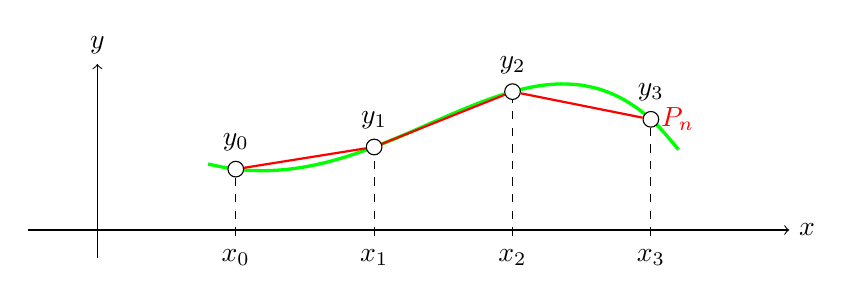
\begin{tikzpicture}[x=50pt,y=20pt]
	\draw[->] (-0.5,0) -- (5,0) node[right] {$x$};
	\draw[->] (0,-0.5) -- (0,3) node[above] {$y$};
	
	\draw[very thick,domain=0.8:4.2,smooth,variable=\x,green] plot ({\x},{2.19805 - 1.84594*\x + 0.64716*\x*\x + 0.150811*\x*\x*\x - 0.0500811*\x*\x*\x*\x});
	
	\node[draw,label=above:{$y_0$},circle, fill=white, inner sep=2pt] (A) at (1,1.1) {};
	\node[draw,label=above:{$y_1$},circle, fill=white, inner sep=2pt] (B) at (2,1.5) {};
	\node[draw,label=above:{$y_2$},circle, fill=white,inner sep=2pt] (C) at (3,2.5) {};
	\node[draw,label=above:{$y_3$},circle, fill=white, inner sep=2pt] (D) at (4,2) {};
	
	\node[label=below:{$x_0$}] at (1,0) {};
	\node[label=below:{$x_1$}] at (2,0) {};
	\node[label=below:{$x_2$}] at (3,0) {};
	\node[label=below:{$x_3$}] at (4,0) {};
	
	\draw[-, dashed] (1,-0.1) -- (A);	
	\draw[-, dashed] (2,-0.1) -- (B);
	\draw[-, dashed] (3,-0.1) -- (C);
	\draw[-, dashed] (4,-0.1) -- (D);
	
	\draw[-,thick,red] (A) -- (B) -- (C) -- (D) node[right] {$P_n$};
	
\end{tikzpicture}
\end{figure}


Entonces, deberíamos tener que

\[ y(x) \equiv \lim_{h\to 0} P_n(x) \]

Es también una solución razonable, pero llegamos a la misma dificultad que antes: no sabemos en qué consiste el límite de una sucesión de funciones.

\subsection{Análisis funcional y sucesiones de funciones}

De cualquiera de las formas tenemos que entrar en análisis funcional, así que tratemos de dar sentido a ese concepto de sucesiones de funciones. Partimos de un conjunto de funciones $\{f_n(x)\}_{n∈ℕ}$ definidas para $x∈(a,b)$. ¿Qué significa entonces el límite $\displaystyle\lim_{n\to ∞} f_n(x) = f(x)$?

Hay varias definiciones para ese límite. La primera es la convergencia puntual:

\subsubsection{Convergencia puntual}

La convergencia puntual consiste en la convergencia de cada uno de los puntos del intervalo. Es decir

\[ f_n\to f \iff \lim_{n\to ∞} f_n(x) = f(x) ∀x ∈ (a,b) \]

O, en términos de ε y δ, que para $x∈(a,b)$

\[ ∀ε>0\, ∃n_0 \st n> n_0 \implies \abs{f_n(x) - f(x)} < ε \]

Ahora bien, hay que leer con cuidado. En esta definición, tenemos que $n_0 = n_0(ε,x)$ depende de dos parámetros. Esta definición es por lo tanto muy débil como para usarla en los métodos de resolución anteriores.

\begin{figure}[hbtp]

\centering
\begin{tikzpicture}[x=150pt, y=30pt]
\draw[->] (-0.1, 0) -- (1.4,0);
\draw[->] (0,-0.1) -- (0,5);

\draw[-,blue, thick] (0,0) -- (0.0625,4) -- node[above right] {$y_n$}  (0.125,0) -- (1.3,0);
\draw[-,red, thick] (0,0) -- (0.25,2) -- node[above right] {$y_2$} (0.5,0) -- (1.3,0);
\draw[-,green, thick] (0,0) -- (0.5,1) -- node[above right] {$y_1$} (1,0) -- (1.3,0);

\node[vnlin, label=below:{$\dfrac{1}{n}$}] at (0.125,0) {};
\node[vnlin, label=below:{$\dfrac{1}{2}$}] at (0.5,0) {};
\node[vnlin, label=below:{$1$}] at (1,0) {};
\end{tikzpicture}
\caption{Sucesión de funciones $y_n$}
\label{imgAF_Yn}
\end{figure}

Consideremos la familia de funciones $y_n$ definidas como en la figura \ref{imgAF_Yn}. Por ejemplo, $\lim_{n\to ∞} y_n(0) = 0$. En $x=\frac{1}{2}$, tenemos 

\[ \{y_n(1/2) \}_{n∈ℕ} = \{ 1,0,0,\dotsc \} \]

y por lo tanto $\lim_{n\to ∞} y_n(1/2) = 0$. En general, para cualquier $x>0$, tendríamos que existe un $n_0$ tal que si $\frac{1}{n_0} < x$ entonces $y_m(x) = 0$ para todo $m≥n_0$. Es decir, que tendríamos una convergencia puntual:

\[ \lim_{n\to ∞} y_n(x) = 0 \; ∀x∈[0,1] \]

Ahora bien, ¿qué ocurre con la integral? Sería igual al área, y entonces

\[ \lim_{n\to ∞} \int_0^1 y_n(x) \dif x = \frac{1}{n} · n ·\frac{1}{2} =\frac{1}{2} \]

pero sin embargo

\[ \int_0^1 \lim_{n\to ∞}y_n(x) \dif x = \int_0^1 0\dif x = 0 \]

Las integrales difieren, no podemos \textit{intercambiar} el límite con la integral y por lo tanto esta definición es muy débil para lo que buscamos. Tenemos que buscar una noción alternativa.

\subsubsection{Convergencia uniforme}

\begin{definition}\name{Convergencia}[uniforme] Diremos que una sucesión de funciones $y_n$ converge uniformemente a $y$ en el intervalo $(a,b)$ si y sólo si $∀ ε > 0 ∃n_0 = n_0(ε)$ tal que si $n>n_0$ entonces

\[ \abs{y_n(x) - y(x)} < ε ∀x∈(a,b) \]

o, dicho de otra forma

\[ \sup_{x∈[a,b]} \abs{y_n(x) - y(x)} < ε \]
\end{definition}

La convergencia uniforme tiene una interpretación geométrica que podemos ver en la figura \ref{imgConvUnif}.

\begin{figure}[hbtp]
\centering
\begin{tikzpicture}[scale=1.5,declare function={
	wav_sl(\x,\ofst) = 0.3 * \x + 1 + \ofst + 0.2 * sin(3 * \x r);
	wav_pert(\x,\a,\b) = \a * cos(7* \x r) + \b * sin(\x r) * cos(\x * 5 r);
}]
\draw[->] (-0.1,0) -- (5,0);
\draw[->] (0,-0.1) -- (0,3);

\fill[draw=none,domain=0.8:4.2,smooth,variable=\x,green!50!white, fill=green!10] 
	(0.8, {wav_sl(0.8,-0.5)}) -- plot ({\x}, {wav_sl(\x,0.5)}) -- (4.2, {wav_sl(4.2,-0.5)})
	plot ({5 - \x}, {wav_sl(5 - \x,-0.5)});


\draw[thick,domain=0.7:4.3,smooth,variable=\x,blue!10] plot ({\x}, {wav_sl(\x,-0.2) + wav_pert(\x,0.15,0.1)});
\draw[thick,domain=0.7:4.3,smooth,variable=\x,blue!20] plot ({\x}, {wav_sl(\x,0.2) + wav_pert(\x,0.132,-0.07)});
\draw[thick,domain=0.7:4.3,smooth,variable=\x,blue!40] plot ({\x}, {wav_sl(\x,0.07) + wav_pert(\x,0.05,-0.01)});
\draw[thick,domain=0.7:4.3,smooth,variable=\x,blue!80] plot ({\x}, {wav_sl(\x,0) + wav_pert(\x,0.01,0.04)});

\draw[very thick,domain=0.8:4.2,smooth,variable=\x,black] plot ({\x}, {wav_sl(\x,0)});
\draw[thick,domain=0.8:4.2,smooth,variable=\x,green!50!white] plot ({\x}, {wav_sl(\x,0.5)});
\draw[thick,domain=0.8:4.2,smooth,variable=\x,green!50!white] plot ({\x}, {wav_sl(\x,-0.5)});


\node[draw, circle, fill=white, inner sep=1.5pt] (M) at (2, {wav_sl(2,0)}) {};
\node[draw, circle, fill=white, inner sep=1.5pt] (U) at (2, {wav_sl(2,0.5)}) {};
\node[draw, circle, fill=white, inner sep=1.5pt] (L) at (2, {wav_sl(2,-0.5)}) {};

\node[hnlin, label=left:{$y(x)$}] (MO) at (0, {wav_sl(2,0)}) {};
\node[hnlin, label=left:{$y(x) + ε$}] (UO) at (0, {wav_sl(2,0.5)}) {};
\node[hnlin, label=left:{$y(x) - ε$}] (LO) at (0, {wav_sl(2,-0.5)}) {};

\draw[-] (U) -- (M) -- (L);

\draw[dashed,gray] (UO) -- (U);
\draw[dashed,gray] (MO) -- (M);
\draw[dashed,gray] (LO) -- (L);
\end{tikzpicture}
\caption{Interpretación geométrica de la convergencia uniforme a $y(x)$ (negro). Todas las $y_n$ (en azul, más oscuro indica $n$ mayor) estarán en la banda coloreada.}
\label{imgConvUnif}
\end{figure}

Si volvemos al ejemplo de los triángulos, vemos que siempre tenemos una punta que se sale fuera de la banda $(-ε, ε)$ para cualquier ε que escojamos.

\paragraph{Propiedades de la convergencia uniforme} Dadas $f_n\to f,\; g_n\to g$

\begin{itemize}
\item $f_n+g_n \to f + g$
\item $f_ng_n \to fg$
\item $\frac{f_n}{g_n} \to \frac{f}{g}$ si $g≠0$.
\end{itemize}

Además de las propiedades algebraicas, tenemos varios teoremas.

\begin{theorem} Sea $\{f_n\}_{n∈ℕ}$ una sucesión de funciones continuas en $(a,b)$. Si $f_n$ converge uniformemente a $f$ en $(a,b)$, entonces $f$ es continua en $(a,b)$.
\end{theorem}

\begin{proof} Queremos probar que dado $x_0∈(a,b)$, $∀ε>0\, ∃δ>0 \st \abs{x-x_0} < δ \implies \abs{f(x) - f(x_0)} < ε$. Conocemos la convergencia uniforme en $(a,b)$.

Sumamos y restamos $f_n(x)$ y $f_n(x_0)$. Entonces

\[ \abs{f(x) - f(x_0)} = \abs{f(x) \pm f_n(x) \pm f_n(x_0) - f(x_0)} ≤ \abs{f(x) - f_n(x)} + \abs{f_n(x) - f_n(x_0)} + \abs{f_n(x_0) - f(x_0)} \]

Podemos elegir $n > n_0$ tal que tanto $\abs{f(x) - f_n(x)}$ como $\abs{f_n(x_0) - f(x_0)}$ sean menor que $\frac{ε}{3}$, por la convergencia uniforme. Sólo falta hacer pequeño el sumando central, y eso lo hacemos usando la continuidad de las $f_n$.
\end{proof}

\begin{theorem} Supongamos que $f_n\to f$ uniformemente en $(a,b)$, con $(a,b)$ intervalo \textbf{acotado}. Entonces

\[ \lim_{n\to ∞} \int_a^b f_n(x) \dif x = \int_a^b \lim_{n\to ∞} f_n(x) \dif x = \int_a^b f(x) \dif x \]
\end{theorem}

\begin{proof} Usamos el teorema del sandwich y acotamos la diferencia de integrales.

\[ 0 ≤ \abs{ \int_a^b f_n(x) \dif x - \int_a^b f(x) \dif x } ≤ \int_a^b \underbrace{\abs{f_n(x) - f(x)}}_A \dif x \]

donde $A$ es menor que $ε$ para todo $x$ si $n>n_0$. Por lo tanto, 

\[ \int_a^b \abs{f_n(x) - f(x)} \dif x < ε(b-a) \]

que se hace tan pequeño como queramos.
\end{proof}

\begin{definition}\name{Sucesión}[de Cauchy uniforme] Se dice que $\{ f_n \}$ es de Cauchy uniforme en $(a,b)$ si y sólo si $∀ε>0$ $∃n_0=n_0(ε)$ tal que si $n,m>n_0$ entonces 

\[ \abs{f_n(x) - f_m(x)} < ε\; ∀x∈(a,b) \]
\end{definition}

\subsubsection{El espacio de las funciones continuas}

Denotamos al espacio $\mathcal{C}([a,b])$ como el conjunto de las funciones continuas en el intervalo $[a,b]$.

\begin{definition}\name{Norma}[de funciones]\label{defNormaFun} Definimos

\[ \norm{f}_{∞} = \sup_{x∈[a,b]} \abs{f(x)} \]
\end{definition}

A partir de la norma definimos la distancia 

\[ d_∞(f,g) = \norm{f-g}_{∞} \]

y por lo tanto tenemos una definición de convergencia de funciones:

\[ f_n \convs[\norm{\cdot}_{∞}] f \iff d_∞(f_n,f) \convs[][n] 0 \]

que es equivalente a la convergencia uniforme.

Uniendo todos estos conceptos, tendríamos que $\mathcal{C}\left([a,b];\norm{\cdot}_{∞}\right)$ es el espacio de las funciones continuas con la topología de la convergencia uniforme.

\footnote{Aquí faltan las clases de dos días. Un teorema de existencia y unicidad global para sistemas lineales con coef. continuos y otro también global para EDO con segundo término globalmente Lipschitz.}

Veíamos ejemplos en los que pedir una función globalmente Lipschitz era pedir demasiado. Por ejemplo, $f(y)=y^2$ no es globalmente Lipschitz. Por lo tanto, buscaremos algo más débil que nos dé teoremas de existencia y unicidad más generales.

\begin{definition}\name{Condición}[de Lipschitz local]  Se dice que $f(x,y)$ es localmente Lipschitz respecto de $y$ en una región $A$ si y sólo si $∀(x_0,y_0)∈A$ existe un rectángulo $R$

\[ R_{(x_0, y_0)} = [x_0-ε,x_0+ε] × [y_0-d, y_0+δ] \]

tal que $R_{(x_0, y_0)}⊆ A$, y una constante $L_R$ tal que 

\[ \abs{f(x,y) - f(x,z)} < L_R\abs{y-z}\quad ∀(x,y),(x,z)∈R_{(x_0, y_0)} \].
\end{definition}

\paragraph{Interpretación geométrica de la condición de Lipschitz local} Consideremos una función de Lipschitz $f$ \[\abs{f(x,y) - f(x,z)} < L\abs{y-z} \] y nos fijamos sólo en la $y$ y en la $z$. Mantenemos $z$ fijo con valor 1 (por ejemplo). Esto entonces acota nuestra función

\begin{gather*}
-L\abs{y-1} ≤ f(y) - f(z) ≤ L\abs{y-1}
\underbrace{f(1) - L \abs{y-1}}_{G(y)} ≤ f(y) ≤ \underbrace{f(1) + L\abs{y-1}}_{H(y)}
\end{gather*}

entre dos funciones $G(y)$ y $H(y)$. Es decir.

\begin{figure}[hbtp]
\centering
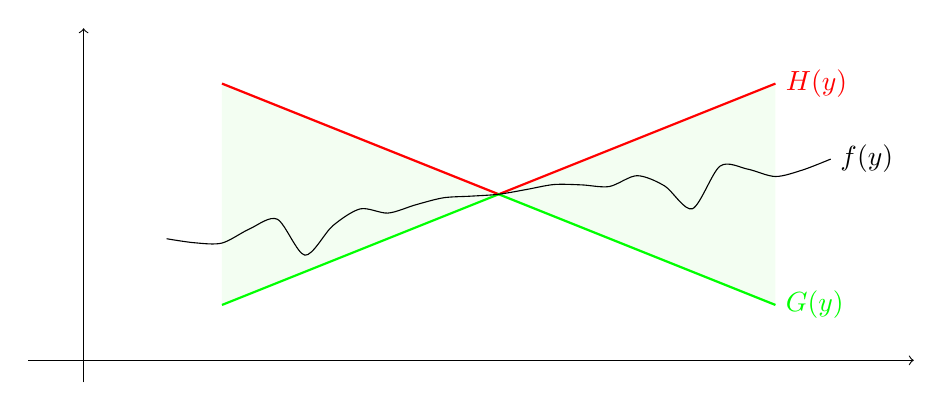
\begin{tikzpicture}[y=40,x=100, declare function={
	wav_sl(\x,\a,\b) = 0.3 * (\x - \a) + \b - 0.1 + 0.1 * cos(20 * pow((\x - \a),2) r) + 0.15 * sin(10 * pow((\x - \a),2) r);
}]
\draw[->] (-0.2, 0) -- (3,0);
\draw[->] (0,-0.2) -- (0,3);

\fill[red!5!green!5] (0.5,2.5) -- (1.5, 1.5) -- (2.5,2.5) -- (2.5,0.5) -- (1.5, 1.5) --  (0.5,0.5);
\draw[thick,-, red] (0.5,2.5) -- (1.5, 1.5) -- (2.5,2.5) node[right] {$H(y)$};
\draw[thick,-, green] (0.5,0.5) -- (1.5, 1.5) -- (2.5,0.5) node[right] {$G(y)$};
\draw[domain=0.3:2.7,smooth,variable=\x,black] plot ({\x},{wav_sl(\x,1.5,1.5)}) node[right] {$f(y)$};
\end{tikzpicture}
\end{figure}

Y lo importante es que lo hace \textbf{en todo el intervalo} que estemos considerando. El mismo cono podemos trasladarlo por la función en todo el intervalo y siempre acotará la función.

En el caso de la raíz cuadrada, vemos que en el 0 vamos a tener una tangente vertical y por lo tanto no vamos a encontrar nunca la constante $L$, ya que tiende a infinito en el cero. Es decir, podemos extraer varias observaciones:

\begin{itemize}
\item Lipschitz implica continua.
\item Lipschitz \textbf{no implica} derivable (p.ej., $\abs{y}$).
\item Derivable \textbf{no implica} Lipschitz global.
\end{itemize}

Parece que podemos encontrar alguna conexión entre Lipschitz y la derivada. Consideramos una $f$ derivable. Entonces 

\[ f(y_1) - f(y_2) = f'(z) (y_1 - y_2) \]

por el teorema del valor medio. Entonces, ese $f'(z)$ sería nuestra constante de Lipschitz $L$. Es decir, la condición de Lipschitz implica acotación de la derivada, que esa $L$ no se va a infinito.

A partir de esta definición podemos llegar a otro nuevo teorema de existencia y unicidad

\begin{theorem}[de existencia y unicidad local] Sea $f(x,y)$ una función continua localmente Lipschitz con respecto a la segunda variable ($y$) en una región $A⊆ℝ^2$ abierta.

Entonces, dado el problema 

\[ \begin{cases}
y'(x) &= f(x,y(x)) \\
y(x_0) &= y_0
\end{cases} \]

con $(x_0, y_0)∈A$, entonces existe una \textbf{única solución local}. Es decir:

\begin{itemize}
\item Existe una constante $α>0$ y una función $y(x)$ que es solución en $[x_0-α, x_0+α]$.
\item Dadas soluciones $y_1$ definida en $[x_0-α_1, x_0+α_1]$, $y_2$ definida en $[x_0-α_2, x_0+α_2]$, ambas son iguales en el intervalo común $[x_0-α_1, x_0+α_1] \cap [x_0-α_2, x_0+α_2]$.
\end{itemize}
\end{theorem}

\begin{proof}
Hay dos formas de llevar a cabo la demostración: o por el teorema de la aplicación contractiva o por el método de iteradas de Picard. Hagamos los dos.

\paragraph{1) T. Aplicación Contractiva} Buscamos demostrar que \[ y(x) = y_0 + \int_{x_0}^x f(s,y(s)) \dif s \] para $x∈[x_0, x_0+h]$.

Trabajaremos en el espacio $X$, el conjunto de funciones $y(x)$ continuas en el intervalo  $[x_0, x_0+h]$ tales que $(x,y(x))∈R_{(x_0, y_0)}\; ∀x∈[x_0, x_0+h]$. 

Definimos la transformación de funciones \[ Ty = y_0 + \int_{x_0}^{x} f(s,y(s)) \dif s \] y buscamos un punto fijo de $T$. Entonces

\[ \abs{Ty(x) - Tz(x)} ≤ \int_{x_0}^{x} \abs{f(s,y(s)) - f(s,z(s))} \dif s \stackrel{\text{Lipschitz}}{≤} \int_{x_0}^x L_R \abs{y(s)-z(s)}\dif s \]

Sabiendo que $\abs{y(s)-z(s)}$ será menor siempre que la norma entre esas dos funciones (ver \ref{defNormaFun}), sustituimos y 

\[ \norm{Ty(x) - Tz(x)}_\infty ≤ L_Rh\norm{y-z}_\infty \]

y por lo tanto será contractivo si $h<\frac{1}{L_R}$.

Sin embargo, el teorema de la aplicación contractiva sólo vale para funciones de un espacio en sí mismo. En este caso, no es seguro que $Ty∈X$. Para poder aplicar el teorema, hay que demostrar que $T$ es una aplicación $\app{T}{X}{X}$. Vamos a ello.

Tenemos que demostrar que si $(x,y(x)) ∈R\; ∀x∈[x_0, x_0+h]$, entonces $(x, Ty(x))∈R\; ∀x∈[x_0, x_0+h]$, o, dicho de otra forma, que $\abs{Ty(x) - y_0}<δ$.  En este caso, vemos que

\[ \abs{Ty(x) - y_0} ≤ \int_{x_0}^x \abs{f(s,y(s))}\dif s \]

Necesitamos que aparezca $y_0$ por alguna razón, así que sumamos y restamos y nos queda 

\[ \abs{Ty(x) - y_0} ≤ \int_{x_0}^x \underbrace{\abs{f(s,y(s))}}_{A} + \underbrace{\abs{f(s,y(s) - f(s,y_0)}}_{B} \dif s \]

Tenemos que $A<C_0$ por ser $f$ continua. Por otro lado, $B<L_R\abs{y-y_0}$ por la condición de Lipschitz, y al estar $y$ en el rectángulo $R$ entonces $B<L_Rδ$. Nos queda entonces 

\[ \abs{Ty(x) - y_0} ≤(C_0 + L_R δ)h \]
y nos bastará tomar $h$ suficientemente pequeño para que se cumpla que $ \abs{Ty(x) - y_0} < δ$, es decir,

\[ h < \frac{δ}{C_0 + L_Rδ} \]

Para finalizar la prueba, nos quedamos con el $h$ mínimo entre este y el que hace que sea contractiva:

\[ h < \min \left\{ \frac{δ}{C_0 + L_Rδ}, \frac{1}{L_R} \right\} \]

\paragraph{2) Iteradas de Picard} Sudo. De hecho

\begin{verbatim}
sudo rual completa esto
\end{verbatim}
\end{proof}

Lo bueno del método de iteradas de Picard es que nos permitirá demostrar un lema adicional de continuidad con respecto a los datos.

\begin{theorem}[de Gronwall] Dada una función 

\[ w(x)≤ h + \int_{x_0}^x k(s)w(s)\dif s \]

con $k$ continua y mayor o igual que cero, entonces 

\[ w(x) ≤ h \exp{\int_{x_0}^xk(s)\dif s} \]
\label{thmGronwall}
\end{theorem}

\begin{proof}

Sea $v(x) = \int_{x_0}^x k(s)w(s)\dif s$. Entonces $v(x_0) = 0$, y  \[ v'(x) = k(x)w(x) \] por el Teorema Fundamental del Cálculo. Sustituyendo de nuevo

\[ v'(x) ≤ k(x) (h + v(x)) = hk(x) + k(x) v(x) \]

Nos queda un sistema

\[ \begin{cases}
v'(x) - k(x)v(x) ≤ hk(x) \\
v(x_0) 
\end{cases} \]

Resolvemos aplicando un factor integrante $μ(x) ≥ 0$. Entonces

\[ μ(x)v'(x) - k(x)μ(x)v(x) ≤ hk(x)μ(x) \] es la ecuación a plantear y nos queda

\begin{gather*}
μ' = -kμ \implies μ(x) = \exp -\int_{x_0}^x k(s) \dif s \\
(μ(x)v(x))' ≤ h k(x) μ(x) \\
(μ(x)v(x))' ≤ -hμ'(x) \\
\int_{x_0}^x (μ(x)v(x))' ≤-h \int_{x_0}^x μ'(s) \dif s 
μ(x)v(x) - \underbrace{μ(x_0) v(x_0)}_0 ≤ -h (μ(x) - \underbrace{μ(x_0)}_1)
\end{gather*}

En total, nos queda

\begin{gather*}
\exp\left(-\int_{x_0}^x k(s)\dif s\right) v(x) ≤ -h \left(\exp\left(-\int_{x_0}^x k(s)\dif s\right) - 1\right) \\
w(x) - h ≤ v(x) ≤ h \left(\exp\left(-\int_{x_0}^x k(s)\dif s\right) - 1\right) \\
w(x) ≤ h \exp\left(-\int_{x_0}^x k(s)\dif s\right) 
\end{gather*}

En un caso más general, si tengo que \[ w(x) ≤ h(x) + \int_{x_0}^x k(s)w(s)\dif s \] con $k$ continua y mayor o igual que cero, llegaríamos a la conclusión haciendo cuentas análogas de que

\[ w(x) ≤ h(x) + \int_{x_0}^x h(s) k(s) e^{\int_{x_0}^xk(t)\dif t} \dif s \]

\end{proof}

Con este lema, podemos construir otro de continuidad respecto de los datos.

\begin{theorem}[Continuidad respecto de los datos]\label{thmContDatos}

Dados dos problemas

\[ \begin{cases}
y'(x) &= f(x,y(x)) \\
y(x_0) &= y_0
\end{cases}, \begin{cases}
z'(x) &= f(x,z(x)) \\
z(x_0) &= z_0
\end{cases} \] con $f$ función Lipschitz, entonces 

\[ \abs{y(x)-z(x)} ≤ \abs{y_0-z_0} M \] con $M∈ℝ$.

Dicho de otra forma, datos próximos nos dan soluciones próximas.
\end{theorem}

\begin{proof}

Dados dos problemas

\[ \begin{cases}
y'(x) &= f(x,y(x)) \\
y(x_0) &= y_0
\end{cases}, \begin{cases}
z'(x) &= f(x,z(x)) \\
z(x_0) &= z_0
\end{cases} \]

tenemos que

\begin{gather*}
y(x) = y_0 + \int_{x_0}^{x} f(s,y(s)) \dif s \\
z(x) = z_0 + \int_{x_0}^{x} f(s,z(s)) \dif s 
\end{gather*}

Entonces, si restamos y tomamos valores absolutos,

\begin{multline*}
 \abs{y(x) - z(x)} ≤ \abs{y_0-z_0} + \int_{x_0}^x \abs{f(s,y(s)) - f(s,z(s))} \dif s \\ \stackrel{\text{Lipschitz}}{≤}  \abs{y_0-z_0} + \int_{x_0}^x L_R\abs{y(s)-z(s)} \dif s \end{multline*}

Podemos aplicar el Lema de Gronwall a esta ecuación:

\[ \underbrace{\abs{y(x) - z(x)}}_{w(x)} ≤ \underbrace{\abs{y_0-z_0}}_{C} + \int_{x_0}^{x} \underbrace{L_R}_{k(s)} \underbrace{\abs{y(s)-z(s)}}_{w(x)} \dif s \]

y entonces tenemos que 

\[ \abs{y(x)-z(x)} ≤ \abs{y_0-z_0}e^{\int_{x_0}^{x}L_R\dif S} = \abs{y_0-z_0} M \]

donde $M$ es una constante, así que tenemos la continuidad.
\end{proof}

\subsection{Ejercicios}

\begin{example} Analiza la convergencia puntual y uniforme de las siguientes sucesiones de funciones.

\begin{enumerate}
\item $f_n(x) = x^n -x^{n+1}$ en $[0,1]$.
\item $f_n(x) = \frac{e^x}{x^n}$ en $(1,∞)$.
\item $f_n(x) = x^n - x^{2n}$ en $[0,1]$.
\item $f_n(x) = n \left(\sqrt{x + \frac{1}{n}} - \sqrt{x}\right)$ en $x > 0$.
\item $f_n(x) = \sin\left(\frac{x}{n}\right)$ con $x∈ℝ$.
\end{enumerate}

\paragraph{$f_n(x) = x^n -x^{n+1}$} Buscamos primero la convergencia puntual, y tenemos que 

\[ \lim_{n\to ∞} x^n-x^{n+1} = 0 \] por lo que converge puntualmente.

Estudiamos ahora la convergencia uniforme con el límite

\[ \lim_{n\to ∞} \max_{x∈[0,1]} \abs{f_n(x) - 0} = \lim_{n\to ∞} \max_{x∈[0,1]} x^n - x^{n+1} \]

Para hallar el máximo, derivamos e igualamos a cero:

\[ nx^{n-1} - (n+1){x^{n-1}} = x^{n-1}(n-(n+1)x) = 0 \] y nos queda 

\[ \lim_{n\to ∞} \max_{x∈[0,1]} f_n(x) = f_n\left(\frac{n}{n+1}\right) = \underbrace{\frac{1}{\left(1+\frac{1}{n}\right)^n}}_{\convs \frac{1}{e}} \cdot \underbrace{\frac{1}{n+1}}_{\convs 0} = 0 \] y por lo tanto hay convergencia uniforme.

\paragraph{$f_n(x) = \frac{e^x}{x^n}$} Puntualmente y con $x>1$

\[ \lim_{n\to ∞} x^{-n} e^x = 0 \]

Estudiamos la convergencia uniforme

\[ \lim_{n\to ∞} \sup_{x>1} \abs{f_n(x)} = \lim_{n\to ∞} \sup_{x>1} x^{-n} e^x \]

Derivamos e igualamos a cero

\[ e^xx^{-n-1}(x-n) = 0 \iff x=n \]

y evaluando

\[ \lim_{n\to ∞} \eval{f_n(x)}_{x=n} = \lim_{n\to ∞} \left(\frac{e}{n}\right)^n = 0 \]

Ojo, porque en este caso no tenemos convergencia uniforme. No hemos demostrado que en $x=n$ haya un máximo: de hecho, es un mínimo. También tendríamos que tener cuidado con el supremo y no el máximo, ya que estamos en un conjunto no acotado.

\paragraph{$f_n(x) = x^n - x^{2n}$} Convergencia puntual. Cero. Uniforme: otra vez lo del límite, puede poner máximo.\footnote{Esta mierda de ejercicio que estoy copiando está patrocinado por la falta de sueño por culpa de redes.} Deriva. Saca algo. Es un máximo. Evalúa, distinto de cero, no hay convergencia uniforme.

\paragraph{$f_n(x) = n \left(\sqrt{x + \frac{1}{n}} - \sqrt{x}\right)$} Hay que hacer el conjugado... se va a algún sitio y $\frac{1}{2\sqrt{x}} = f(x)$ es el límite puntual. Vamos a la uniforme y miramos si converge al límite puntual

\[ \lim_{n\to ∞} \sup_{x∈(0,∞)} \abs{f_n(x) - f(x)} \]

pero ese uno entre dos raíz de equis se va a menos infinito, y como tenemos hun balor havzolutoh me ahorro las dos caras de cuentas de derivadas de Azorero. Pero dice que no, que comprobemos en $(1/2, + ∞)$.

\paragraph{ $f_n(x) = \sin\left(\frac{x}{n}\right)$} Parece que sí hay convergencia puntual. No hay uniforme en todo $ℝ$ ya que habrá algún valor en el que el seno valga uno. Sin embargo, en un intervalo acotado sí habrá convergencia uniforme.
\end{example}


\begin{example} Determinar para qué valores de $α≥0$ se satisface una condición de Lipschitz con respecto de $y$ siendo 

\[ f(x) = \abs{y}^α \].

Es trivial ver que para $α=0,1$, se cumple. Para valores mayores que 1, la derivada estará acotada si estudiamos la condición en intervalos acotados. Si $α<1$, tendremos problemas en el 0.

La filosofía es que raíces malas en el 0, potencias malas en el infinito.

Supongamos $y>0$, entonces $f'(y) = α y^{α-1}$. Para $α>1$, 

\[ \abs{f(y_1)-f(y_2)} \stackrel{TVM}{=} \abs{f'(z)} \abs{y_1-y_2} = αz^{α-1} \abs{y_1-y_2} \stackrel{?}{<} L \abs{y_1-y_2} \]

y entonces debe ser $αz^{α-1}<L$, es decir, tenemos que tener una cuota superior para $y_2$.
\end{example}


\subsection{Diferenciabilidad con respecto a los datos}

Hasta ahora hemos estado viendo problemas de la forma

\[ \begin{cases}
y' = f(x,y) \\
y(x_0) = t
\end{cases} \]. 

En realidad, al resolver, obtenemos funciones $y(x,t)$, una familia de soluciones que dependen del valor inicial de $t$. 

Sabemos que si $f(x,y)$ es continua y localmente Lipschitz en un abierto $A⊆ℝ^2$ con $(x_0,t)∈A$, entonces tenemos existencia y unicidad local.

Por otro lado, también demostramos un resultado de continuidad con respecto a los datos. Es decir, $y(x,t)$ es continua con respecto a $t$ (ver lema \ref{thmContDatos}). 

El paso siguiente es ver qué ocurre cuando $f$ es algo \textit{mejor} que Lipschitz: $y(x,t)$ será también \textit{mejor}. Veamos el teorema:

\begin{theorem}[Diferenciabilidad respecto a los datos] Si $f$ es una función continua en $x$ y además $C^1$ con respecto a la segunda variable, entonces la solución $y(x,t)$ es derivable respecto de $t$.
\end{theorem}

\begin{proof} Fijamos $t$, y estudiamos el límite que representa la derivada

\[ \lim_{h\to 0} \frac{y(x,t+h) - y(x,t)}{h} = \lim_{h\to 0} P_h(x) \]

Dicho de otra forma,

\[ P_h(x) = \frac{1}{h}\left((t+h) + \int_{x_0}^x f(s, y(s, t+h)\dif s - t - \int_{x_0}^x f(s, y(s, t)\dif s\right) \] 
que no es más que la reformulación usando la forma integral de $y$. Si seguimos operando

\[ P_h(x) = 1 + \int_{x_0}^x\frac{1}{h}\left(f(s, y(s,t+h)) - f(s,y(s,t+h))\right)\dif s \]

Si aplicamos el teorema del valor medio

\[ P_h(x) = 1 + \int_{x_0^x} \underbrace{\pd{f}{y}(s,z(s,h))}_{F}\underbrace{\frac{1}{h} (y(s,t+h) - y(s,t))}_{P_h(x)} \dif s \]

con $z(s,h)$ un valor intermedio entre $y(s,t)$ e $y(s,t+h)$, que tiende a $y(s,t)$ cuando $h\to 0$. Llamamos $F$ a la derivada parcial para simplificar, y además vemos que nos vuelve a salir $P_h$. Reescribimos

\[ P = 1 + \int_{x_0}^{x} FP \dif s \]
y vemos que estamos antes la formulación integral del siguiente problema

\[ \begin{cases}
P' = FP \\
P(x_0) = 1
\end{cases} \implies P = e^{\int_{x_0}^x F\dif s} \]

Calculamos ahora el límite de $P_h$ cuando $h\to 0$. El punto delicado es cómo pasar el límite de fuera de la integral a dentro. Asumiendo que se puede hacer sin problemas, quedaría

\[ \lim_{h\to 0} P_h(x) = \exp{\int_{x_0}^x \pd{f}{y}(s,y(s,t)) \dif s} = \pd{y}{t} \]

Para poder pasar el límite, tenemos que tener convergencia uniforme. Como estamos trabajando en un conjunto compacto con una función continua, la función es uniformemente continua , tendremos esa convergencia y podremos pasar el límite dentro.

\end{proof}

\subsection{Resultados de prolongabilidad}

Queremos explorar hasta dónde llegan las soluciones que obtenemos y el tipo de desastres que podemos encontrar. Tenemos el problema de siempre,

\[ \begin{cases}
y' = f(x,y) \\
y(x_0) = t
\end{cases} \], con $f(x,y)$ es continua y localmente Lipschitz en un abierto $A⊆ℝ^2$ con $(x_0,t)∈A$, entonces tenemos existencia y unicidad local.

Sabemos varias cosas:

\begin{itemize}
\item \textbf{Existencia local} $∃α>0, y(x)$ solución definida en $[x_0,x_0 + α]$.
\item \textbf{Unicidad} Si tenemos dos soluciones $y_1,y_2$ definidas en los intervalos $[x_0, x_0 + α_{1/2}]$ respectivamente, entonces ambas son iguales en el intervalo $[x_0, x_0 + \min \{α_1,α_2\}]$.
\end{itemize}

La pregunta es, ¿hay una solución maximal, que no se pueda extender más? Consideremos el conjunto

\[ S= \{ α∈ℝ \st ∃ y(x) \text{ solución en } [x_0,x_0+α] \} \]

Buscamos $α_{max} = \sup S$, que nos dará el intervalo maximal $[x_0, x_0 + α_{max})$. Es importante tener en cuenta que el intervalo está abierto por la derecha. 

Lo primero que tenemos que considerar es que en el intervalo maximal no puede haber dos soluciones distintas que arranquen del mismo punto. 

Si nos salimos fuera del conjunto $A$ en el que la función es Lipschitz, podemos tener un desastre. ¿Qué puede ocurrir dentro?

Podemos tener una solución que \textit{se pare antes}, que oscile infinitamente, que llegue al borde o que explote.\footnote{Dibujitos}

El teorema nos dice que las primeras dos cosas no pueden ocurrir, y que las dos segundas sí. Esta cosa tan vaga la formalizamos viendo que toda solución se escapa de cualquier conjunto compacto estrictamente contenido en $A$ y que contenga al dato inicial. 

\begin{theorem}
Consideramos el problema
\[ \begin{cases}
y' &=f(x,y) \\ 
y(x_0)&=y_0
\end{cases} \]
con $f$ continua y localmente Lipschitz respecto de $y$ en un abierto $A\subset \real^2$ con $(x_0,y_0)\in A$. 

Entonces para cualquier compacto K con $(x_0,y_0)\in K\subset A$, podemos encontrar $x^{\ast}\in[x_0,x_0+\alpha_{max})$ tal que $(x^{\ast},y(x^{\ast}))\in A-K$.


\end{theorem}

\begin{proof}
Llamamos $S\equiv \{\alpha\in\real \st \text{ la solución y(x) está definida en } [x_0,x_0+\alpha] \}$ y $\alpha_{max} = sup(s)$.

$\forall n>0$ podemos encontrar $x_n \in \left(x_0 + \alpha_{max} - \frac{1}{n},x_0+\alpha_{max}\right)$ tal que $s_n\in S$, donde 

Entonces podremos construir una sucesión $x_n$ creciente de Cauchy cuyo límite es $x_0+\alpha_{max}$ en $x_0 + \alpha_{max}$ tal que y esté definida en todos los $x_n$.

Vamos a demostrarlo por \textbf{reducción al absurdo:}

Supongamos $(x,y(x))\subset K, \forall x\in[x_0,x_0+\alpha_{max}]$.

En particular $\{(x_n,y(x_n))\}\subset K$,


Entonces queremos ver que $| y(x_n) - y(x_m)|$ para comprobar si es convergente y si tiene límite utilizando el criterio de Cauchy.

Poniendolo en notación integral:

\[| y(x_n) - y(x_m)| \underset{m>n}{=} y_0 + \int_{x_n}^{x_m} f(s,y(s))ds \leq M |x_m-x_n| \]

\paragraph{Conclusión:}
Por ser $\{X_n\}$ convergente, entonces $\{y(x_n)\}$ es de Cauchy y por tanto tiene límite, que vamos a llamar $y^{\ast}$ .

Como K es compacto, entonces $y^{\ast}\in K$. (por ser límite de la sucesión).

¿Podemos definir $y(x_0+\alpha_{max} = y^{\ast})$? 
\textbf{Respuesta:} Todavía no. Si tuvieramos una solución que oscile al acercarse a la frontera, el límite dependería de la sucesión que eligiéramos. Necesitamos demostrar que $y^{\ast}$ no depende de la sucesión $\{x_n\}$ de puntos de la curva que hayamos elegido.

Para ello: sea $\{z_n\}$ ptra sucesión con $z_n$ que se aproxima a $x_0+\alpha_{max}$. ¿Qué pasa con $|y(x_n) - y(z_n)| \to 0$? 


\[|y(x_n) - y(z_n)| = \int_{x_n}^{z_n} f(s,y(s))ds \underset{\begin{array}{c}(x,y(x))\in K \subset A\\\text{ f continua }\end{array}}{\leq}M |z_n - x_n| \to 0 \implies (*) \]
\[(*) \implies \exists!y^{\ast} \st y^{\ast} = \lim_{x\to (x_0+\alpha_{max})^{-}} y(x) \text{ para cualquier sucesión con límite } x_0+\alpha_{max}\]


Estudiamos este problema:
\[\begin{array}{cc}
y' &= f(x,y)\\
y(x_0+\alpha_{max} &= y^{\ast})
\end{array}\]
Por ser Lipschitz tenemos el teorema de existencia y unicidad local (refrencia) entonces tendríamos una solución que sobrepase el punto $x_0+\alpha_{max}$ contradiciendo la hipótesis.

\end{proof}

Algunas estimaciones del intervalo maximal. 

Vamos a considerar $A \equiv (x,b)×ℝ$, es decir, una banda vertical en $\real^2$.

\paragraph{Caso 1}
Supongamos que la $f(x,y)\leq C,\forall (x,y)\in A$ (está acotada). Además suponemos (como siempre) que $f$ es continua y localmente Lipschitz.

Tenemos un $(x_0,y_0)$ y queremos comprobar si la solución llega al extremo (o por el contrario tiene una asíntota).

Sea la solución: $\displaystyle y(x) = y_0 + \int_{x_0}^{x} f(s,y(s))ds\, x\int [x_0,x_0+\alpha_{max})\subset [x_0,b)$.

\[y(x) - y_0| \leq \int_{x_0}^x |f(s,y(s))|ds \leq C |x-x_0|\]

\[y(x) - y_0|\leq C |x-x_0| \implies y_0 - C(x-x_0) \leq y(x) \leq y_0 + C(x - x_0)\] es decir, está controlada por las rectas $y_0 \pm C(x-x_0)$ evitando así cualquier asíntota vertical. Además, el teorema anterior nos dice que la solución se sale del conjunto compacto, con lo que el intervalo maximal llega hasta b.

\textbf{Lado derecho acotado implica solución global en (a,b)}

\paragraph{Caso 2} Supongamos $|f(x,y)|\leq A(x)|y| + B(x);\, A,B\ge 0$ continuas en (a,b)

Trabajando con notación integral:
\[|y(x)| \leq  |y_0| + \int_{x_0}^x | A(s)|y(s)| + B(s)|ds = \underbrace{|y_0| + \int_{x_0}^x B(s)ds}_{C} + \int_{x_0}^x A(s)|y(s)|ds \]
Esta es una desigualdad que nos permite aplicar el lema de Gronwall.

Entonces $|y(x)| \leq C \exp{\int_{x_0}^{b^{\ast}} A(s)ds }$.

Donde $b^{\ast}$ es un punto arbitrario para acotar la solución con un valor que no dependa de $x$.

\textbf{El intervalo maximal $\equiv (a,b)$}


\paragraph{Ejemplo:} 
\[\begin{array}{cc}
y'&=y^2\\
y(0)&=1
\end{array}\]

\[\frac{y'}{y^2} = 1 ; \int_0^x \frac{y'/s(ds)}{(y(s))^2} = \int_0^x 1ds = x \implies ... \implies y(x) = \frac{1}{1-x}\]
Aquí el intervalo maximal hacia la derecha es $[0,1)$.

Sin embargo, el lado derecho ($y^2$) es localmente Lipschizt en todo $\real^2$.

Vamos a demostrarlo para recordar: Siendo una función derivable, aplicamos que si la derivada está acotada, entonces la primitiva el Lipstchizt. 

Como $2y$ es localmente acotada, entonces $y^2$ es localmente Lipschitz.

Vamos a definir un compacto $K = [0,R]×[1,1+h]$ y por el teorema anterior sabemos que la solución se escapa del compacto. Ahora vamos a ver si por arriba o por la derecha (para ver hasta donde llega el intervalo maximal).

\[0\leq y' \leq (1+h)^2\]
Integrando, (con alguna cuenta intermedia) obtenemos:
\[1\leq y (x) = 1 + (1+h)^2 x\]

Es decir, la solución está acotada por 2 rectras, $y=1$ por abajo y $1 + (1+h)^2 x$ por arriba (hasta el corte con el borde superior del compacto, que llamamos $R(h)$).

Lo único que podemos decir es que la solución no ha \textit{explotado} antes de $R(h)$.

Vamos a calcular (creo que por diversión) cuánto vale $R(h)$.
\[(1+h) = (1+h)^2x+1\]
\[R(h) = \frac{h}{(1+h)^2}\]


No era por diversión. Si tenemos $h\to \infty$ ó $h=0 \implies R(h) \to 0$. Esto nos da un máximo: $h=1; R(1)=\frac{1}{4}$.

\textbf{Conclusión} el intervalo de existencia contiene a $\left[0,\frac{1}{4}\right]$.

El dibujo de los triángulos te lo dejo a ti Rual xD

Haciendo el apaño de los triángulos llegamos a un intervalo $\left[0,\frac{1}{2}\right]$

Vamos a ver un ejemplo más sencillo por el que tendríamos que haber empezado (tal vez) q estoy muy cansado como para copiar........

\footnote{Quince primeros minutos de clase faltan aquí}

\begin{example}
Veamos el problema \[ \begin{cases} y' &= y^{2/3} \\ y(0) &= 0 \end{cases} \]

No podemos aplicar directamente el teorema de existencia y unicidad: la derivada no está acotada alrededor de 0 y por lo tanto no es localmente Lipschitz en ese punto. Si nos dijeran que $y(0) = ε ≠ 0$ sí sería localmente Lipschitz en un entorno pequeño del punto.

Como no podemos aplicar el teorema, tenemos que estudiar el caso más detenidamente. En primer lugar, vemos que $y\equiv 0$ es solución. También podemos resolver como una ecuación de variables separadas:

\[ \int_0^x \frac{y(s)}{y^{2/3}(s)} \dif s = \int_0^x \dif s = x \] sobre la que podemos hacer un cambio de variables $y(s) = t$, $y'(s) \dif s = \dif t$ y entonces

\[ \int_{y(0)}^{y(x)} \frac{\dif t}{t^{2/3}} = \eval{t^{1/3}{\frac{1}{3}}}_{t=y(0)=0}^{y(x)} = 3y^{1/3}(x) 
\] 
y por lo tanto \[ y(x) = \left(\frac{x}{3}\right)^3 \] es otra solución.

¿Hay alguna más? Efectivamente, de hecho podemos combinar las dos:

\[ y(x) = \begin{cases}
0 & x ≤ 0 \\
\left(\frac{x}{3}\right)^3 & x > 0
\end{cases}\quad \text{\'o} \quad y(x) = \begin{cases}
\left(\frac{x}{3}\right)^3 & x ≤ 0 \\
0 & x ≤ 0\end{cases} \]

E incluso podemos conseguir infinitas soluciones combinando "desplazamientos", como por ejemplo el de la figura \ref{imgInfSoluciones}.
\end{example}

\begin{figure}[hbtp]
\centering
\begin{tikzpicture}
\draw[->] (-3,0) -- (3,0);
\draw[->] (0,-3) -- (0,3);

\draw[thick,domain=-2.8:1,smooth,variable=\x,blue!80] plot ({\x}, {0});
\draw[thick,domain=1:2.8,smooth,variable=\x,blue!80] plot ({\x}, {(\x-1)*(\x-1)*(\x-1)/3});
\end{tikzpicture}
\label{imgInfSoluciones}
\caption{Una solución posible trasladando otra con dato inicial $y(1) = 0$}
\end{figure}


Sin embargo, no tiene por qué ocurrir siempre que se nos descuadre todo al no poder aplicar la condición de Lipschitz. Veamos otro ejemplo

\begin{example}
 \[ \begin{cases} y' &= (y-x)^{2/3} \\ y(x_0) &= y_0 \end{cases} \]
 
 En este caso los problemas aparecen cuando $y=x$. Es decir, que podemos aplicar el teorema de existencia y unicidad local cuando $y_0 ≠ x_0$. 
 
 Supongamos, por poner las cosas interesantes, que $y(1) = 1$. Hay que estudiar este caso directamente.
 
 Podemos resolverlo a través del teorema de la función implícita. Sea $w(x) = y - x$. Haciendo las sustituciones
 
 \begin{gather*}
 y(x) = w(x) + x \\
 y' = w' + 1
 \end{gather*} 
 
 convertimos el problema en 
 
 \[ \begin{cases}
 w'+1 = w^{2/3} \\
 w(1)  = 0
 \end{cases} \]
 
 Resolviendo como ecuación de variables separadas de la misma forma que en el anterior ejemplo, llegamos a la integral
 
 \[ \int_{0}^{w(x)}  \frac{\dif t}{t^{2/3} - 1} \]
 
 Y ahí está la solución, si pudiésemos resolver explícitamente la integral y despejar $w$. Pero podemos usar el teorema de la función implícita. Tenemos una función $F$ definida como
 
 \[ F(x,w) = (x-1) - \int_{0}^{w(x)}  \frac{\dif t}{t^{2/3} - 1} 
 \] 
 con $F(1,0) = 0$. ¿Podemos despejar $w(x)$? Para saberlo necesitamos comprobar que la derivada es distinta de cero:
 
 \[ \pd{F}{w} = - \eval{\frac{1}{w^{2/3} - 1}}_{(x,w) = (1,0)} = 1 ≠ 0 \] y por lo tanto el TFI nos dice que existe $w(x)$ despejable a partir de $F$ y que además es única.
\end{example}

En resumidas cuentas, cuando no se cumplen las hipótesis del teorema puede pasar cualquier cosa. Veamos otro ejemplo bastante artificial pero interesante.

\begin{example}
\[ \begin{cases}
y' &= \frac{\sqrt{1-y^2}}{1+x^2} \\
y(0) = \frac{1}{2}
\end{cases} \]

La ecuación nos restringe $y$ al intervalo $[-1,1]$ para que la raíz cuadrada esté definida. Y de hecho, en esos dos extremos del intervalo la derivada será cero así que tendremos un problema. Por otra parte, $y\equiv \pm 1$ son soluciones de la ecuación (no del problema entero).

La solución es

\[ y(x) = \sin \left(\frac{1}{1-x} - 1 + \frac{π}{4}\right) 
\]
que no es más que una traslación de la función $\sin\frac{1}{1-x}$, cuya gráfica se ve en la figura \ref{imgSenoOsc}. En $1$ tenemos un montón de oscilaciones, por lo tanto el intervalo maximal de la solución será $[0, 1)$.
\end{example}

\begin{figure}[hbtp]
\centering
\includegraphics[width=0.8\textwidth]{img/SenoOscilaciones.png}
\caption{$y(x) = \sin\frac{1}{1-x}$}
\label{imgSenoOsc}
\end{figure}

\begin{example} 

\[ \begin{cases}
y' = \dfrac{x^2 + 4y^2 + xy}{1 + x^2 + y^2} \\
y(x_0) = y_0
\end{cases} \]

Se verifica condición de Lipschitz local y por lo tanto tenemos existencia y unicidad local para cualquier punto $(x_0,y_0)$. ¿Hasta dónde llega la solución?

Podemos aplicar uno de los tres casos que hemos visto. Los dos polinomios son del mismo orden, por lo tanto el lado derecho estará acotado y tendremos el primer caso, de tal forma que tenemos existencia global.

Vamos a demostrar mejor la existencia de esa cota.

\begin{multline*}
 \dfrac{x^2 + 4y^2 + xy}{1 + x^2 + y^2} ≤ \dfrac{x^2 + y^2 + 3y^2 + \abs{xy}}{1 + x^2 + y^2} ≤ \dfrac{1 + x^2 + y^2 + 3 y^2 + xy}{1 + x^2 + y^2} =\\ =
  1 + \frac{3y^2 + \abs{xy}}{1+x^2+y^2} ≤ 1 + \frac{3(1+x^2+y^2) + \abs{xy}}{1+x^2+y^2} = 4 + \frac{\abs{xy}}{1+x^2+y^2} \end{multline*}

Por último, viendo que $0≤(x-y)^2 = y^2+x^2 - 2xy \implies \dfrac{x^2+y^2}{2} ≥ xy$ nos queda que 

\[ 
	4 + \frac{\abs{xy}}{1+x^2+y^2} ≤ 4 + \frac{x^2+y^2}{2(1+x^2+y^2)} ≤ 4 + \frac{1 x^2+y^2}{2(1+x^2+y^2)} = 4 + \frac{1}{2} 
\]
y, efectivamente, nos queda una cota.


\end{example}

En muchos casos nos encontraremos cálculos complicados, y en estos casos podemos usar argumentos de comparación con problemas más simples. Veamos cómo hacerlo.

\begin{example}
\[ \begin{cases} 
y' = y^2 +x^2 \\
y(0) = 1
\end{cases} \]

A pesar de la sencillez de la ecuación, resolverla será difícil. Podemos explorar ecuaciones similares. Por ejemplo, viendo que el dato inicial nos lo dan en $x=0$, podemos pensar que la ecuación deberá parecerse mucho a 

\[ \begin{cases} 
z' = z^2 \\ 
z(0) = 1
\end{cases} \].


\begin{wrapfigure}{r}{0.4\textwidth}
\centering
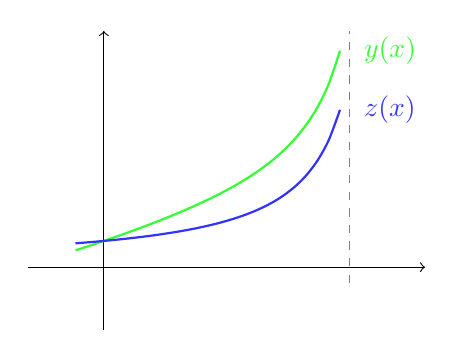
\begin{tikzpicture}[xscale=1.2]
\draw[->] (-0.8,0) -- (3.4,0);
\draw[->] (0,-0.8) -- (0,3);

\draw[thick,domain=-0.3:2.5,smooth,variable=\x,green!80] plot ({\x}, {1/(3-\x) + 0.3*\x})  node[right,xshift=5pt] {$y(x)$};
\draw[thick,domain=-0.3:2.5,smooth,variable=\x,blue!80] plot ({\x}, {1/(3-\x)}) node[right,xshift=5pt] {$z(x)$};
\draw[dashed, gray] (2.6,-0.2) -- (2.6, 3);
\end{tikzpicture}
\caption{Gráfica de $y(x)$ y $z(x)$.}
\label{imgGraficaAprox}
\end{wrapfigure}

Vemos que la gráfica de $z$ se mantendrá por debajo todo el tiempo, ya que $z' < y'$ en todo caso (ver figura \ref{imgGraficaAprox}). Como la solución del segundo problema es $z(t) = \dfrac{1}{1-t}$, $y$ también tendrá una asíntota vertical en $t=1$ o incluso antes. Por lo tanto, el intervalo maximal a la derecha para $y(t)$ está contenido en $(0,1)$.

También podemos llegar al mismo resultado de otra forma, trabajando con desigualdades. Sabiendo que $y$ es siempre mayor que cero, podemos decir

\[ y'= y^2+x^2 ≥ y^2 \implies \frac{y'}{y^2} ≥ 1 \]

Integrando
\[
 \int_0^x \frac{y'(s)}{y^2(s)}\dif s ≥ \int_0^x \dif s = x
\] 
y haciendo cambio de variable $y(s) = t$, $y'(s)\dif s = \dif t$
\[ 
\int_1^{y(x)}\frac{\dif t}{t^2} = \eval{\frac{-1}{t}}_{t=1}^{y(x)} = 1 - \frac{1}{y(x)}
\].

Con esto nos quedaría la siguiente desigualdad.

\[ y(x) ≥ \frac{1}{1-x} \].

También podemos hacer una segunda estimación. Aplicando que el intervalo maximal de nuestra solución es como  mucho $(0,1)$, vemos que
\[ 
y' = y^2 + x^2 ≤ y^2 + 1
\]
lo que nos daría una nueva estimación

\[ y(x) ≤ \tan\left(x + \frac{π}{4}\right) \].

Juntando todos los resultados, tendríamos una estimación como la de la figura \ref{imgEstRegion}.

\end{example}


\begin{figure}[hbtp]
\centering
\begin{tikzpicture}[xscale=1.5, yscale=1.2]
\draw[->] (-0.8,0) -- (3.4,0);
\draw[->] (0,-0.8) -- (0,3);

\draw[thick,domain=-0.3:0.6,smooth,variable=\x,green!80] plot ({\x}, {tan((\x + pi/4) r) / 2}) node[right,xshift=5pt] {$\tan\left(x + \dfrac{π}{4}\right)$};
\draw[thick,domain=-0.3:2.5,smooth,variable=\x,blue!80] plot ({\x}, {1/(3-\x)}) node[right,xshift=5pt] {$\dfrac{1}{1-x}$};
\draw[dashed, gray] (2.6,-0.1) -- (2.6, 3);
\draw[dashed, gray] (0.65,-0.1) -- (0.65, 3);
\node[label=below:{$\dfrac{π}{4}$}] at (0.65,0) {};
\node[label=below:{$1$}] at (2.6,0) {};

\end{tikzpicture}
\caption{La función real $y(x)$ estará entre las dos funciones que hemos estimado..}
\label{imgEstRegion}
\end{figure}

\paragraph{Método de las poligonales de Euler y funciones no-Lipschitz} Consideremos el ejemplo anterior de $y'=y^{2/3}$. Si aplicamos el método de las poligonales de Euler, no encontraríamos ninguna otra solución que no fuese la constante $y\equiv 0$. Sin embargo, si tomamos un punto inicial $y(0) = ε$ la solución sí crecerá. Por lo tanto, si no tenemos un teorema que nos garantice unicidad tendremos que estudiar qué ocurre alrededor de ese punto para comprobar que no nos dejamos ecuaciones.

Sigamos con más ejemplos.


\begin{figure}[hbtp]
\centering
\begin{tikzpicture}[xscale=2,yscale=1.4]

\draw[->] (-0.8,0) -- (3,0);
\draw[->] (0,-0.8) -- (0,2);

\draw[gray,-,fill=orange!10] (0,0) rectangle (2,1);
\draw[pattern=horizontal lines, pattern color=red!70!orange] (0,0) -- (0.86,1) -- (2,1) -- (2,0) -- (0,0);
\path[name path=hl] (0,1) -- (2,1);
\draw[name path=fn, very thick,-] (-0.5,-0.6) -- (1.5,1.8) node[right] {$(h^4+r)x$};

\path [name intersections={of=hl and fn,by=E}];
\node (I) [above=0.5 of E] {};
\node (IO) [below=1 of E] {};
\draw[dashed] (I) -- (IO);
\node[vnlin,label=below:{$R(h)$},anchor=north] at (IO) {};

\node[anchor=north west,orange!80!black] at (0,1) {$K$};
\node[hnlin,gray,label=left:{$h$}] at (0,1) {};
\node[vnlin,gray,label=below:{$R$}] at (2,0) {};
\end{tikzpicture}
\caption{Representación del conjunto $K$, donde la zona rayada es donde encontraremos la solución.}
\label{figConjuntoK}
\end{figure}

\begin{example}
\[ \begin{cases}
y' = y^4 + r \\
y(0) = 0
\end{cases}
\] 
con $r>0$. La ecuación verifica una condición de Lipschitz local. A primera vista vemos que $y'>0$ y por lo tanto $y≥0$.

Consideramos el conjunto $K$, un rectángulo de altura $h$ y anchura $R$ (figura \ref{figConjuntoK}). Podemos hacer una estimación y operar

\begin{gather*}
0 ≤ y^4 + r ≤ h^4 + r \\
0 ≤ y' ≤ h^4 + r \\
0 ≤ y(x) ≤ (h^4+r)x \quad ∀(x,y) ∈ K
\end{gather*}

Por lo tanto, la solución tendrá un intervalo maximal a la derecha $[0,b)$, donde $b$ será mayor o igual a $R(h)$, que es la intersección de la recta $(h^4+r)x$ con $y=h$, es decir

\[ R(h) = \frac{h}{h^4+r} \]

Queremos hallar el $R(h)$ óptimo, así que derivando y operando obtenemos que

\[ b ≥ R(h_{max}) = \left(\frac{r}{3}\right)^{-3/4} \frac{1}{4} \]

Tomemos ahora la indicación del problema. Suponemos que $b>r^{-3/4}$. ¿Qué estimación podemos obtener a partir de esto? 
\end{example}



\begin{example}[Problema 16]
Tenemos 

\[ \begin{cases}
y' = \frac{y}{1+x^2} + e^{-y^2} \\
y(0) = 10
\end{cases},\quad 
\begin{cases}
z' = \frac{z}{1+x^2} \\
z(0) = 10
\end{cases} \]

Queremos demostrar que $0< y(x) - z(x) ≤ e^{-100} (e^x-1)$.

En el caso de la primera ecuación, vemos que $y'≥0$, así que $y(x) ≥ 10\,∀x ≥ 0$. Además, $f(x,y)$ es continua en $ℝ^2$. Para comprobar la condición de Lipschitz, acotamos

\[ \abs{\pd{f}{y}} = \abs{\frac{1}{1+x^2}+e^{y^2}(-2y)} ≤ \frac{1}{1+x^2} + 2\abs{y} e^{-y^2} ≤ 1+2\abs{y} 
\] 
y tenemos condición de Lipschitz local, por lo que tenemos existencia y unicidad local. Además, también podemos acotar el lado derecho de la ecuación por un término lineal:

\[ \abs{f(x,y)} ≤ \abs{\frac{y}{1+x^2} + e^{-y^2}} ≤ \frac{\abs{y}}{1+x^2} + e^{-y^2} ≤ \abs{y} + 1 
\]
lo que, junto con el segundo teorema de prolongabilidad, tenemos existencia en $[a,b]$  $∀a,b$.

Pero además, podríamos haber logrado una cota mejor para $2\abs{y} e^{-y^2}$. Sabiendo que es una función continua y que tiende a 0 cuando $y\to \infty$, podemos decir que existe un máximo $C$. Acotando esa parte por una constante tendríamos Lipschitz global y existencia en todo $ℝ$ de la solución.

Pasamos ahora al segundo problema. Es una ecuación de variables separadas, así que integramos (podemos pasar la $z$ dividiendo ya que es siempre positiva):

\begin{align*}
\frac{z'}{z} &= \frac{1}{1+x^2} \\
\eval{\log z(s)}_{s=0}^x &= \eval{\arctan s}_{s=0}^x \\
\log z(x) - \log 10 &= \arctan x \\
z(x) &= 10 e^{\arctan x}
\end{align*}

De hecho, si aplicamos esto al primer problema, podemos decir que

\begin{align*}
y' &>  \frac{y}{1+x^2} \\
\frac{y'}{y} &> \frac{1}{1+x^2} \\
y(x) &> 10 e^{\arctan x} = z(x)
\end{align*}

Tenemos ya la primera parte de la desigualdad, $y(x) - z(x) > 0$. Pasamos a demostrar la segunda parte. Sabemos que
\begin{gather*}
y(x) = 10 + \int_0^x \frac{y(s)}{1+s^2} + e^{-y^2(s)} \dif s \\
z(x) = 10 + \int_0^x \frac{z(s)}{1+s^2} \dif s \\
y(x) - z(x) = \int_0^x \frac{y(s)-z(s)}{1+s^2} + e^{-y^2(s)} \dif s
\end{gather*}.

Transformamos la ecuación para aplicar el lema de Gronwall (\ref{thmGronwall}):

\( \label{eqProb16}
y(x) - z(x) = \int_0^x e^{-y^2(s)} \dif s + \int_0^x \frac{y(s)-z(s)}{1+s^2}\dif s ≤ e^{-100} + \int_0^x \frac{y(s)-z(s)}{1+s^2}\dif
\)
Tomando $k(s) = \frac{1}{1+s^2}$, nos quedaría que 
\[ 
y(x) - z(x) ≤ e^{-100}e^{\int_0^x\frac{1}{1+s^2}\dif s} = e^{-100} e^{\arctan x} 
\].

Comparamos con lo que nos pedían: hemos llegado a algo parecido pero no a lo mismo. De hecho, cuando $x\to 0$ la exponencial es mejor en la desigualdad que nos daban, y es que el Lema de Gronwall nos va a dar siempre el mismo resultado: cuando $x\to 0$, la integral se va a cero y por lo tanto la cota se quedaría en $e^{-100}$.

Lo que haremos será parar antes de la primera estimación, en \eqref{eqProb16}, y ver qué cuentas hacíamos en la demostración del lema de Gronwall para no perder precisión. Llamamos $w=y-z$, y 

\[ \int_0^x\frac{w(s)}{1+s^2}\dif s \equiv Φ(x) 
\]. 

Operando:

\begin{gather*}
Φ'(x) = \frac{w(x)}{1+x^2} ≤ \frac{1}{1+x^2}\left(e^{-100} x + Φ(x)\right) \\
Φ'(x) - \frac{1}{1+x^2}Φ(x) ≤ e^{-100}\frac{x}{1+x^2} 
\end{gather*}

Tratamos de resolver esa ecuación diferencial usando un factor integrante $μ≥0$:

\begin{align*}
 μΦ' - \frac{μ}{1+x^2}Φ &≤ e^{-100}μ\frac{x}{1+x^2} \\
 μΦ' + μ'Φ &= μΦ' - \frac{μ}{1+x^2}Φ \\
 μ' &= \frac{-μ}{1+x^2} \\
 \cdots & \cdots \\
 μ(x) &= e^{-\arctan x} \\
\left(e^{-\arctan x}Φ\right)' & ≤ e^{-100} \frac{e^{-\arctan x}x}{1+x^2} \\
\int_0^x \left(e^{-\arctan s}Φ(s)\right)'\dif s &≤ e^{-100}\int_0^x \frac{e^{-\arctan s}s}{1+s^2} \dif s \\
e^{-\arctan x} Φ(x) - 0 &≤ e^{-100} \left( \eval{se^{-\arctan s}}_{s=0}^x + \int_0^x e^{-\arctan s} \dif s \right) \\
Φ(x) &≤ e^{-100}\left(-x+e^{\arctan x}\int_0^2 e^{-\arctan s}\dif s\right)
\end{align*}

Metiendo ahí la estimación de $w≤e^{-100}x + Φ(x)$ (que no sé de dónde puñetas ha salido) tenemos que

\[ w(x) ≤ e^{-100} \left(e^{\arctan x} \int_0^x e^{-\arctan s} \dif s\right) \]

¿Cómo llegamos a que  $e^{\arctan x} \int_0^x e^{-\arctan s} \dif s < e^x -1$? Vemos que para $x∈[0,1]$, $e^{\arctan x} < e^x$ y que como $e^{-\arctan s} < 1$, entonces $\int_0^x e^{-\arctan s} < x$. Sin embargo, esta estimación no es válida. Vamos por otra parte.

Consideramos la función \[ u(x) = e^{\arctan x} \int_{0}^{x}e^{-\arctan s}\dif \]. Si derivamos, 

\begin{gather*}
 u' = \frac{e^{\arctan x}}{1+x^2}\int_0^x e^{-\arctan s}\dif s + e^{\arctan x}e^{-\arctan x} \\
 u' = \frac{u}{1+x^2} + 1 ≤ u+1
 \end{gather*}
 
Resolvemos esta ecuación diferencial con el valor inicial $u(0) = 0$ y nos queda que $u(x) ≤ e^x-1$, y tendríamos resuelto el problema. Pero hemos llegado a prácticamente la misma ecuación que antes, quitándonos el $e^{-y^2}$. Y es que efectivamente, si restamos

\[ (y-z)' = \frac{y-z}{1+x^2} + e^{-y^2} \stackrel{y ≥ 10}{≤} \frac{y-z}{1+x^2} + e^{-100}  ≤ (y-z) + e^{-100} 
\]
y ahora resolviendo \[ \begin{cases} w' ≤ w + e^{-100} \\ w(0) = 0 \end{cases} \implies w(x) ≤ e^{-100}\left(e^x - 1\right) \].
\end{example}